%------------------------------------------------
\begin{frame}
\frametitle{Definition - cryptage, encrypt, encryption ?}

\begin{block}{Encryption}
\justifying{
Encryption is to encrypt a document / file using an encryption key.
The reverse operation is decryption.
}
\end{block}
\begin{block}{Cryptage}
\justifying{
Term « cryptage » is derived from the English encryption and does not exist in French.
Decryption is the fact of breaking the encryption when the private key is unknown.
}
\end{block}
\begin{block}{Cryptography}
\justifying{
Science is called Cryptography.
}
\end{block}
\end{frame}

%------------------------------------------------
\begin{frame}
\frametitle{Encryption, how does it work?}

\begin{block}{Symetric Encryption}
\justifying{
This involves encrypting a message with the same key that will be used for decryption process.
\\
Sample : Caesar code,  with an offset letter. A->C, B->D etc.
\\
Nous venons en paix ->  Pqwu xgpqpu gp rckz
\\
The reverse process is applied to get the message.
}
\end{block}

\begin{block}{What is an encryption key?}
\justifying{

A key is called so because it opens / closes the padlock that is the used encryption algorithm.
\begin {itemize}
\item Here, the algorithm is the offset.
\item The key is the number of offset of letter (here two letters).
\end{itemize}
}
\end{block}

\end{frame}

%------------------------------------------------
\begin{frame}
\frametitle{Asymetric Encryption 1/2}

\begin{block}{Public key - Private key}
\justifying{

Asymetric Encryption is based on the pair public key - private key.
\\$\Rightarrow$ What you need to know: 
\begin{itemize}
\item My private key is... private and my own.
\item My public key is shared with everyone.
\end{itemize}
}
\end{block}
	
\begin{block}{The encryption algorithm}
\justifying{
The encryption algorithm is more complexe than the fact of shifting letters ; it is based on mathematical concepts (first number ...)
}
\end{block}

\end{frame}

\begin{frame}
\frametitle{Asymetric Encryption 2/2}

\begin{block}{Encryption}
With the public key of my correspondent, I encrypt a file.
\justifying{
\\$\Rightarrow$ The file can only be decrypted by the person who possesses the private key corresponding to the public key that I used (and therefore my correspondent).
}
\end{block}

\begin{block}{Decryption}
With its private key, my correspondent decrypts the file.
\\
$\Rightarrow$ He can then read the message.
\end{block}

\begin{block}{Concret case}
Mail Encryption with PGP.
\end{block}
\end{frame}

%----------------------------------------------------------------------------------------
\begin{frame}
\frametitle{Bob send a message to Alice}
\begin{center}
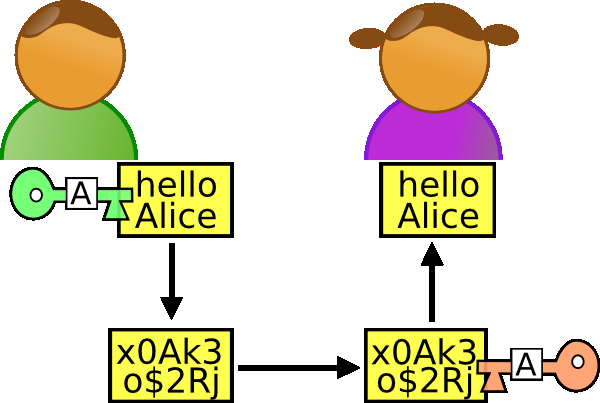
\includegraphics[scale=0.3] {./materials/Alice_et_bob} 
\end{center}
\end{frame}


%----------------------------------------------------------------------------------------
\begin{frame}
\Huge{\centerline{Why encryption?}}
\begin{center}
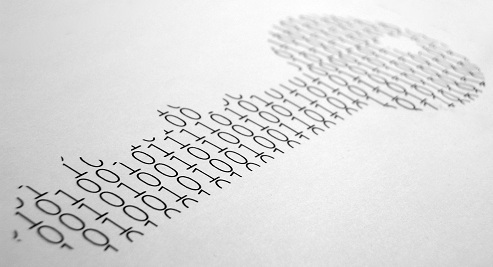
\includegraphics[scale=0.4] {./materials/cryptography.jpg} 
\end{center}
\end{frame}

%------------------------------------------------
\begin{frame}
\frametitle{Encrypt - The arguments against}

\justifying{
\begin{block}{Nobody does...}
FALSE. Without knowing it, you do it every day.
\\
Sample 1: "padlock" when connecting (https)
\\ Sample 2: Wifi key.
\end{block}

\begin{block}{Nothing to hide...}
FALSE. Who would accept the postman read his medical post ?
\end{block}

\begin{block}{Encryption, it's for the pedo-nazi...}
\justifying{
FALSE. For journalists / bloggers dissidents who are denouncing dictatorships...
}
\end{block}
}
\end{frame}

%------------------------------------------------
\begin{frame}
\frametitle{Encrypt - The arguments for}

\begin{block}{Encryption, it's not so complicated}
It is not more complicated than using a "software". You just have to understand the principle.
\end{block}

\begin{block}{Protection and security}
My personnal data are safe Cf. PRISM, NSA...
\end{block}

\begin{block}{Privacy}
Only the person for who the "message" is, is able to read it.
\end{block}

\end{frame}

%----------------------------------------------------------------------------------------
\begin{frame}
\frametitle{Edward Snowden}
\justifying{
Encryption works. Properly implemented strong crypto systems are one of the few things that you can rely on.
}
\begin{center}
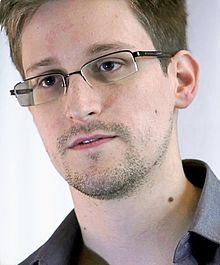
\includegraphics[scale=0.4] {./materials/snowden.jpg} 
\end{center}

\end{frame}


%------------------------------------------------
\begin{frame}
\frametitle{Encryption limit}
\begin{block}{Which is encrypted can be decrypted today tomorrow}
\justifying{
Tomorrow's computers will allow to decrypt the encrypted data today.
}
\end{block}

\begin{block}{It the private key is lost}
We no longer have access to data.
\end{block}

\begin{block}{Metadata, social graph}
\justifying{
\textbf{PGP does not protect against the analysis of metadata (servers transit, addresses, headers, subject).}
Do not forget to clean the meta-data files (EXIF tag photos, office documents with tracked changes).
DNS... Case of tracking Internet ...}
\end{block}

\end{frame}

%----------------------------------------------------------------------------------------
\begin{frame}
\frametitle{Law and encryption}
\justifying{
In France, the law therefore considers that the use of cryptology is free (LCEN Article 30-1) and there is therefore now no limit to the size of the encryption key that can be used .
\\~\\
In case of search, the refusal of submission of the encryption key may result in 3 years imprisonment and 45000\euro{}.
\\~\\
This penalty is increased if Encryption was used to commit a crime.
\\~\\
It is therefore recommended to give the decryption key, except in the case where the decrypted data would result in a judicial proceeding in which the final sentence would be greater than the interference with the judicial investigation.
}
\end{frame}

